\chapter{Heterogeneous Knowledge Graph Construction}
\label{chap:kg}

\section{Motivation: Why a Heterogeneous Graph?}
\label{sec:kg_motivation}

Each cleaned case JSON from Chapter~\ref{chap:pipeline} already carries
typed entities, rhetorical-role-segmented text, and an outcome label.
A flat document representation discards two things this structure
provides. It collapses typed objects, a court, a statute, a
provision, a party, into a single token stream that a model has to
re-disambiguate from scratch, and it has no mechanism to exchange
information \emph{between} cases that share the same statute or
precedent: when two cases both cite IPC~498A, a flat view sees the
string twice while a graph view sees two cases attached to the same
shared node, where one round of message passing can move information
from one to the other. A heterogeneous graph captures both properties
by design: distinct node and edge types preserve typed semantics, and
shared entity nodes provide cross-case conduits. The rest of this
chapter describes the schema, the leakage-prevention strategy, and the
text-embedding features attached to each node.

\section{Graph Schema}
\label{sec:graph_schema}

The graph is constructed as a \textbf{full-star global graph}: every
case is a local "star" of text and entity nodes anchored on a
\textsc{Case} node, and a selected set of entity types are
\emph{shared} across cases so that stars of different cases are
stitched into one connected component.

\subsection{Node Types}

The reasoning-focused graph keeps \textbf{17 node types} in three
categories:

\begin{sloppypar}
\begin{itemize}
  \item \textbf{The case node.} A single \textsc{Case} node per case,
    whose attributes store the outcome label, bucket, filing and
    decision dates (used for temporal gating), and bookkeeping
    metadata.
  \item \textbf{Text nodes.} Six types -- \textsc{Preamble},
    \textsc{Facts}, \textsc{Arguments},
    \textsc{Petitioner\_Arguments}, \textsc{Respondent\_Arguments},
    and \textsc{Other\_Lawyer\_Arguments} -- each carrying a
    \texttt{bge-m3} text embedding of the cleaned, leakage-filtered
    span they represent (Section~\ref{sec:text_features}).
  \item \textbf{Entity nodes.} Ten types: \textsc{Petitioner},
    \textsc{Respondent}, \textsc{Petitioner\_Lawyer},
    \textsc{Defence\_Lawyer}, \textsc{Lawyer}, \textsc{Court},
    \textsc{Judge}, \textsc{Statute}, \textsc{Provision}, and
    \textsc{Precedent}.
\end{itemize}
\end{sloppypar}

Four auxiliary NER types that OpenNyAI produces -- \textsc{Org},
\textsc{GPE}, \textsc{Date}, and \textsc{Case\_Number} -- are
deliberately omitted from the reasoning-focused graph. They carry
little predictive signal for the outcome and would otherwise inflate
the node count and introduce weak, noisy edges that dilute message
passing.

\subsection{Cross-Case Sharing}

Whether two cases share a node, or each hold a private copy of one,
determines whether a GNN can use that node as a cross-case conduit.
The policy is deliberate:

\begin{itemize}
  \item \textbf{Shared across cases}: \textsc{Statute},
    \textsc{Provision}, and \textsc{Precedent}. These are the
    \emph{law itself} -- citing IPC~420 in one case and IPC~420 in
    another is meant to be the same object, and sharing the node is
    what lets the GNN propagate information along the citation.
  \item \textbf{Local to each case}: everything else, including
    \textsc{Court}, \textsc{Judge}, and all \textsc{Lawyer}
    variants. These are \emph{identity proxies}: if a particular
    judge or a particular bench has a historical win/loss bias,
    sharing the node would let the GNN recover that bias as a free
    shortcut to the outcome -- exactly the kind of spurious signal
    the experimental design in Chapter~\ref{chap:results} is built
    to prevent. Keeping them local makes the model reason about the
    law, not about the docket.
\end{itemize}

\subsection{Edges and Graph Structure}
\label{sec:graph_visualizations}

Edges in the schema fall into three groups, summarised in
Table~\ref{tab:edge_groups}: \emph{structural} edges anchoring text
and entity nodes to their parent \textsc{Case}, \emph{citation} edges
forming the legal backbone, and \emph{counsel--argument} edges tying
each lawyer and party to their own argument block. Citations attach
to the \textsc{Arguments} node rather than the case so that a
reference sits in the discourse context of the side that invoked it,
and the provision hierarchy is preserved by
\textsc{Provision}--\textsc{Statute} edges so a citation to
Section~482 sits two hops from the IPC rather than disconnected from
it. Every edge is added in both directions so HGT's message passing
can deliver neighbour information back to the case representation
that the classifier reads.

\begin{table}[H]
  \centering
  \small
  \begin{tabular}{@{}L{2.6cm}L{9.5cm}@{}}
    \toprule
    Group & Edges \\
    \midrule
    Structural
      & \textsc{Case}--text (preamble / facts / arguments /
        petitioner / respondent / other-lawyer arguments);
        \textsc{Case}--party; \textsc{Case}--court;
        \textsc{Case}--judge; \textsc{Case}--lawyer (each role). \\
    Citation
      & \textsc{Arguments}--\textsc{Statute};
        \textsc{Arguments}--\textsc{Provision};
        \textsc{Arguments}--\textsc{Precedent};
        \textsc{Provision}--\textsc{Statute} hierarchy. \\
    Counsel /
    party
      & \textsc{Petitioner\_Lawyer}--\textsc{Petitioner\_Arguments};
        \textsc{Defence\_Lawyer}--\textsc{Respondent\_Arguments};
        \textsc{Lawyer}--\textsc{Other\_Lawyer\_Arguments};
        party--matching-argument-block. \\
    \bottomrule
  \end{tabular}
  \caption{Edge groups in the reasoning-focused schema. Every edge is
  added in both directions.}
  \label{tab:edge_groups}
\end{table}

Figure~\ref{fig:single_case_graph} illustrates the local ``star-graph''
structure surrounding a single \textsc{Case} node, with the citation
edges from the \textsc{Arguments} node fanning out to shared statutes,
provisions, and precedents. These citation edges are constrained
chronologically: a precedent edge is added only when
$\text{precedent\_year} < \text{case\_year}$, and a statute edge only
when $\text{statute\_year} \leq \text{case\_year}$, so a case can never
structurally link forward to authorities that did not exist at the time
it was decided.

\begin{figure}[htbp]
    \centering
    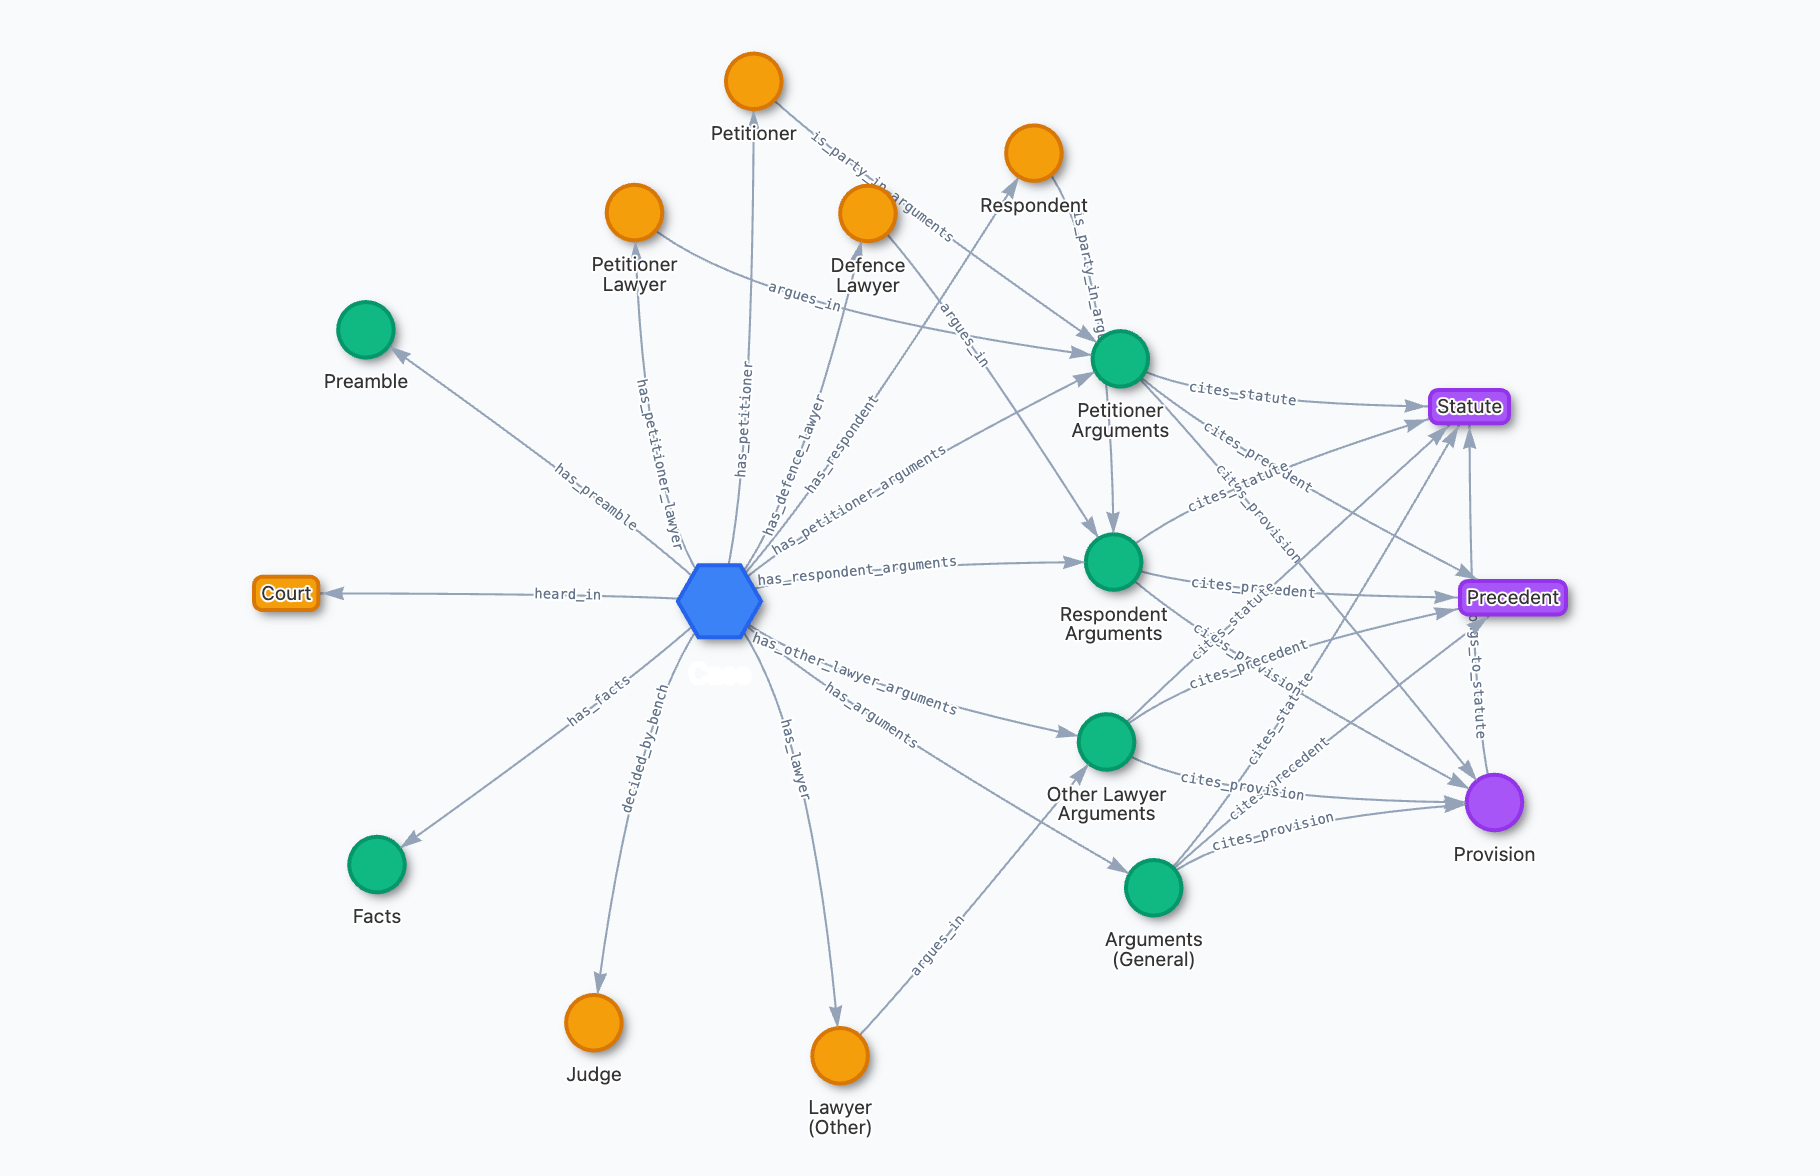
\includegraphics[width=\textwidth]{new_slide_figures/legal_graph_ontology.png}
    \caption{Star-graph structure for a single \textsc{Case} node. Text
    blocks attach as text nodes; identity entities (\textsc{Court},
    \textsc{Judge}, \textsc{Lawyer}) attach as local entity nodes. The
    \textsc{Arguments} node carries the citation backbone out to
    shared \textsc{Statute} and \textsc{Precedent} nodes.}
    \label{fig:single_case_graph}
\end{figure}

Figure~\ref{fig:cross_case_graph} shows how those shared nodes connect
multiple cases into one graph. Statutes, provisions, and precedents
act as cross-case conduits along which the GNN can propagate
information; courts, judges, and individual lawyers are kept private to
each case so that docket-level identity cannot leak the outcome.

\begin{figure}[htbp]
    \centering
    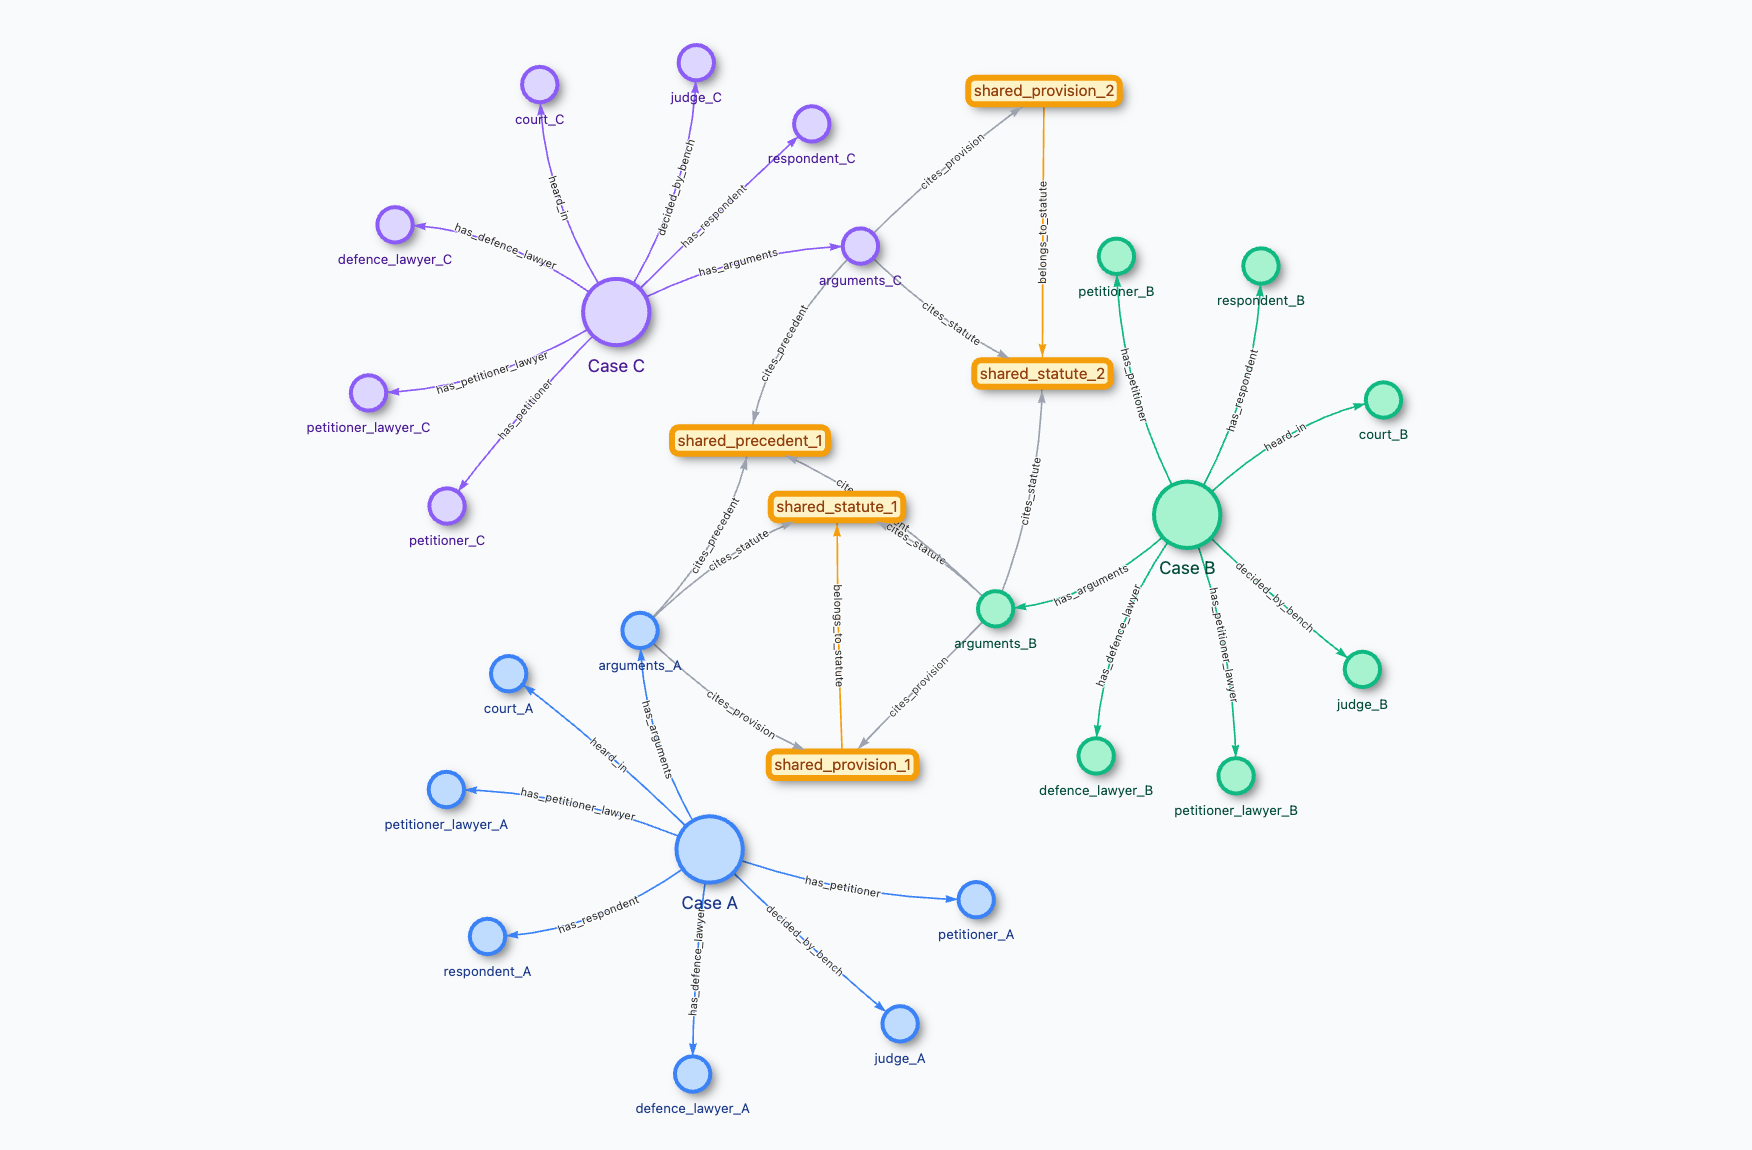
\includegraphics[width=\textwidth]{new_slide_figures/cross_case_graph.png}
    \caption{Cross-case connection through shared legal authorities.
    Identity entities remain local; statutes, provisions, and
    precedents form the cross-case conduits used for message passing.}
    \label{fig:cross_case_graph}
\end{figure}

Each \textsc{Case} node carries its outcome label, bucket membership,
and the dates needed for temporal gating; text nodes carry their
\texttt{bge-m3} embedding (Section~\ref{sec:text_features}); entity
nodes carry their canonical name. Edges are typed with their relation,
which is what the HGT layers use to index their per-relation
parameters (Chapter~\ref{chap:results}).

\section{Leakage Prevention Strategy}
\label{sec:leakage_prevention}

Legal judgment prediction has a notorious failure mode: models that
appear to predict the outcome are in fact \emph{reading} it. A graph
built straight from the OpenNyAI output would expose the verdict
through several distinct channels, top-level outcome fields written
by the labeller, decisive rhetorical-role spans (\textsc{RPC},
\textsc{RLC}), residual decision phrases buried inside otherwise
non-decisive sentences, and shared \textsc{Precedent} or
\textsc{Statute} nodes that link a case to authorities decided after
it. Each of these is closed off explicitly before the graph is
materialised.

\paragraph{Field-level removal.} The cleaning stage strips every
top-level field that contains, scores, or paraphrases the outcome,
the case outcome label, the outcome score, the labeller's confidence
and short explanation, the raw model response, the extracted decision
text, and the cached \textsc{RPC} sentences, along with the
\textsc{decision} block of the OpenNyAI summary. After this step no
case record retains a field that names its own verdict.

\paragraph{Rhetorical-role filtering.} The two decisive role labels,
\textsc{RPC} (the court's operative paragraph) and \textsc{RLC} (the
ruling by the lower court), are dropped together with any annotation
whose label string matches a small blacklist (\texttt{decision},
\texttt{disposition}, \texttt{operative}, \texttt{order},
\texttt{rpc}). This is the single most important gate: without it the
\textsc{Arguments} text node would contain the verdict verbatim.

\paragraph{Phrase-level masking.} Decisive language can survive role
filtering when it is embedded inside a \textsc{Facts} or
\textsc{Arguments} sentence rather than tagged as \textsc{RPC}. A
curated list of outcome-bearing phrases,
\emph{``petition stands disposed of''},
\emph{``appeal is allowed''},
\emph{``set aside''},
\emph{``quashed''}, and so on, is therefore applied as a
case-insensitive, whitespace-tolerant scrubber across every retained
text field, replacing each match with a \texttt{[LEAKAGE\_MASK]} token.

\paragraph{Temporal gating on shared entities.} A shared
\textsc{Precedent} or \textsc{Statute} node would leak future
information if a citation edge were attached to a case decided before
the cited authority existed. The graph builder enforces a strict rule:
a precedent edge is added only when
$\text{precedent\_year} < \text{case\_year}$, and a statute edge only
when $\text{statute\_year} \leq \text{case\_year}$. Cross-case
information therefore flows only along legally honest paths.

\paragraph{Audit trail.} Every case carries a \texttt{leakage\_audit}
record listing the fields dropped, annotations removed, decision text
removed, and phrase-level masks applied. The audit is stored alongside
the graph cache so that any future claim of leakage can be checked
against the per-case ledger rather than argued in the abstract.

Together these gates leave the GNN with a strictly pre-decision view
of the dispute, the parties, the facts, what each side argued, and
the law they invoked, with the verdict itself systematically
withheld.

\section{Text Embedding and Feature Extraction}
\label{sec:text_features}

\subsection{The \texttt{bge-m3} Text Encoder}

All text nodes are featurised with \path{BAAI/bge-m3}, a multilingual
sentence-transformer with a $1024$-dimensional output, run through the
\texttt{sentence\_transformers} library. The choice of \texttt{bge-m3}
is driven by two concrete requirements: (i) Indian legal text mixes
English with Hindi and regional-language transliterations, Latin-script
legal abbreviations, and citation fragments, and \texttt{bge-m3}'s
multilingual training data handles this noticeably better than
English-only encoders; and (ii) the model is strong in retrieval
settings, which aligns with the graph's use of embeddings as
comparison features across cases.

\paragraph{Configuration.} The encoder is run with
\texttt{batch\_size=16}, \texttt{max\_length=512}

\paragraph{Hierarchical chunking for long spans.} Legal judgment
\emph{Facts} and \emph{Arguments} sections routinely exceed the
model's $512$-token window. For texts longer than the configured
character limit, the encoder splits them into overlapping,
sentence-boundary-aligned chunks, encodes each chunk independently,
and mean-pools the resulting vectors. This preserves a consistent
$1024$-dimensional representation per text node regardless of input
length, while avoiding the information loss of a hard truncation.

\paragraph{Caching.} Embeddings are cached per namespace with a
deterministic hash of the input ids, texts, and encoder configuration.


\subsection{Node Feature Assembly}

For each node type the final per-node feature vector is the
concatenation of:

\begin{sloppypar}
\begin{itemize}
  \item the $1024$-dim \texttt{bge-m3} embedding of the node's canonical
    text (for text nodes, that is the full span; for entity nodes,
    that is the canonical name);
  \item scalar node-level features: local frequency in the case,
    section-of-first-mention indicators (\texttt{seen\_in\_preamble},
    \texttt{seen\_in\_arguments}), type one-hot, and for shared entity
    types the log global frequency across the corpus;
  \item for the \textsc{Case} node, bucket one-hot and the outcome
    label is attached only as the supervision target, never as a
    feature.
\end{itemize}
\end{sloppypar}

Because different node types carry different feature dimensionalities,
the HGT model used in Chapter~\ref{chap:results} begins with a
per-node-type linear projection (\texttt{input\_projections}) that maps
all features into a common hidden dimension before the first
heterogeneous message-passing layer. This is the mechanism that lets
the graph remain genuinely heterogeneous at the feature level while
still admitting a uniform message-passing computation.
